\documentclass[12pt,a4paper]{report}
\usepackage[portuguese]{babel}
\usepackage[utf8]{inputenc}
\usepackage{graphicx}\usepackage{hyperref}
\usepackage{acronym}
\begin{document}\title{PL - Processamento de Linguagens \\ Report 2007: vamos escrever relatórios }\date{14 Maio 2014 }
\author{David Angelis   60990    \\Lucas Oliveira   60990    \\Rui Mendes   60990    \\}\maketitle\textbf{\textit{Uminho }}\section*{KeyWords}
\textbf{Yacc }
\textbf{Flex }
\begin{abstract}
Neste trabalho temos como objetivo criar um analisador léxico e um sintático, que processa e analisa o texto,
apanhando as palavras reservadas, e de seguida verifica se a estrutura do relatório está bem construida. Enquando analisa o 
texto vai guardando-o em estruturas de dados, em listas ligadas.E por fim convertendo o nosso relatório em HTML e em LaTex. 
\end{abstract}
\tableofcontents
\listoffigures
\chapter{Introdução }
Para o segundo Trabalho Prático da Unidade Curricular de Processamento de Linguagens, a nossa escolha foi o enunciado 5 que tem como titulo: Report 2007: vamos escrever relatórios. Neste projeto, pretende-se que seja criado um compilador capaz de 
converter
 uma relatório escrito numa linguagem criada por nó. Portanto, neste documento irão estar presentes as nossas decisões, a estruturação do projecto, bem como as explicações e funcionamento do mesmo.
\chapter{Sintaxe da Nossa Linguagem }
A seguinte figura mostra as diferentes palavras reservadas que o analisador léxico deverá reconhecer e comunica-lá ao analisador sintático.   
\begin{figure}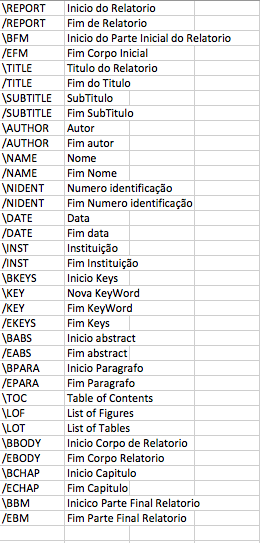
\includegraphics{sintaxe.jpg}\caption{Sintaxe da nossa Linguagem }\end{figure}\chapter{Estrutura do Trabalho }
Este trabalho consiste em dois analisadores, um lexico, feito em flex que irá 
apanhar
 as palavras reservadas na nossa linguaguem e passar a informação do que reconheceu para o analisador sintático, feito em yacc, que irá verificar se a gramática obtida do documento que está a ser analisado está correta.
Depois disto, e no yacc, gravamos os dados em estruturas de dados. Por fim, vamos buscar os dados a essas estruturas e criamos um ficheiro HTML e
ou LaTeX com a nossa linguagem convertida para essas linguagens.
\section{Report }
\begin{verbatim}typedef struct sReport{
Front front;
ListChapter listchapter;
ListaParagraph final;
}*Report,SReport;  
\end{verbatim}Essa estrutura permite-nos representar o relatório que será composto por 3 partes, o FrontMatter, o Body e por ultimo o BackMatter.   
\section{FrontMatter }
\begin{verbatim}
typedef struct sFrontMatter
{
    
char *title;
char *SubTitle;
char *Date;
char *Institution;
ListAuthor lauthor;
ListaParagraph abstract;
ListaParagraph aknowledgement;
KeyWords words;
char *toc;
char *lof;
char *lot;
}*Front, SFront; 
 
\end{verbatim}Essa estrutura será composto por varias identidades e será responsável pela primeira parte do relatório.  
\begin{itemize}\item Titulo do Relatório  \item SubTitulo \item Data \item Instituição \item Lista dos diferentes autores \item Um abstract  \item Agradecimentos  \item Lista de KeyWords  \end{itemize}\section{ListChapter }
\begin{verbatim}
typedef struct sLChapter{
    Capitulo capitulo;
    struct sLChapter *seg;
}*ListChapter,ChapterNodo;
 
\end{verbatim}A struct ListChapter representa uma lista de capítulos que servirá para podermos representar os diferentes capítulos do relatório. 
\section{Capitulo }
\begin{verbatim}
typedef struct SCapitulo{
    char *title;
    LChapter capitulo;
}*Capitulo,Scapitulo;
 
\end{verbatim}A estrutura Capitulo permitirá a representação do capitulo e será composto por um titulo e uma lista ligada de conteúdo que será apresentada de seguida. 
\section{LCapitulo ChapterConteudo }
\begin{verbatim}
typedef struct sChapterConteudo{
    int tipo;
    union{
        ListaConteudo paragraph;
        Float foat;
        ItemList list;
        CodeBlock codeBlock;
        Section section;
        LSumary sumary;
    }ChapConteudo;
}*ChapterConteudo,ChapterConteudoNodo;

typedef struct SLCapitulo{
    ChapterConteudo conteudo;
    struct SLCapitulo *seg;
}*LChapter,Schapter; 
 
\end{verbatim}Essas duas estruturas representam uma lista de conteúdo onde cada nodo da lista poderá ser de diferentes tipos, como era preciso o capitulo aceitar vários tipos decidiu-se criar a estrutura ChapterConteudo com uma union, assim conseguimos resolver esse problema.       
As seguintes estruturas seguem extatamente a mesma arquitetura e não serão apresentada no nosso relatório
\begin{itemize}\item SubSubSection  \item SubSection  \item Section \item ItemList  \item ListConteudo  \end{itemize}\chapter{Conclusão}
Este trabalho prático permitiu-nos consolidar os conhecimentos obtidos nas aulas uma vez que precisamos de tudo o que temos vindo a dar, a forma como estruturar o compilador, como funcionava a gramática disponibilizada pelo docente, o que era suposto os analisadores lexico e semantico fazerem, como funcionavam e interagiam. O nível de dificuldade neste trabalho foi um pouco maior que no primeiro, o que era de esperar, e foi facilitado pelo facto de termos já grande parte da gramática, apenas tendo de fazer algumas alterações. A nossa satisfação perante o que foi produzido neste trabalho é positiva, uma vez que ficamos a perceber melhor a estruturação do compilador dividindo o analisador em analisador lexico e sintatico, colocando depois um programa em C a fazer a gestão dos dados e escrever nos ficheiros HTML e LaTeX nas respetivas linguagens. 
 
\end{document}